\documentclass[tikz,border=2mm]{standalone}
\usetikzlibrary{arrows.meta,automata,calc,intersections,positioning,shapes.callouts,shapes.geometric,3d,arrows,backgrounds,decorations.pathmorphing,fit,matrix,scopes,shadows,shapes,shapes.symbols,mindmap}

\newcommand{\robot}[2]{%
  \filldraw[draw=red,fill=red!20] (#1) circle(5mm);
  \draw[draw=red,->,-Stealth,rotate around={#2:(#1)}] (#1) -- +(5mm,0);}

\begin{document}
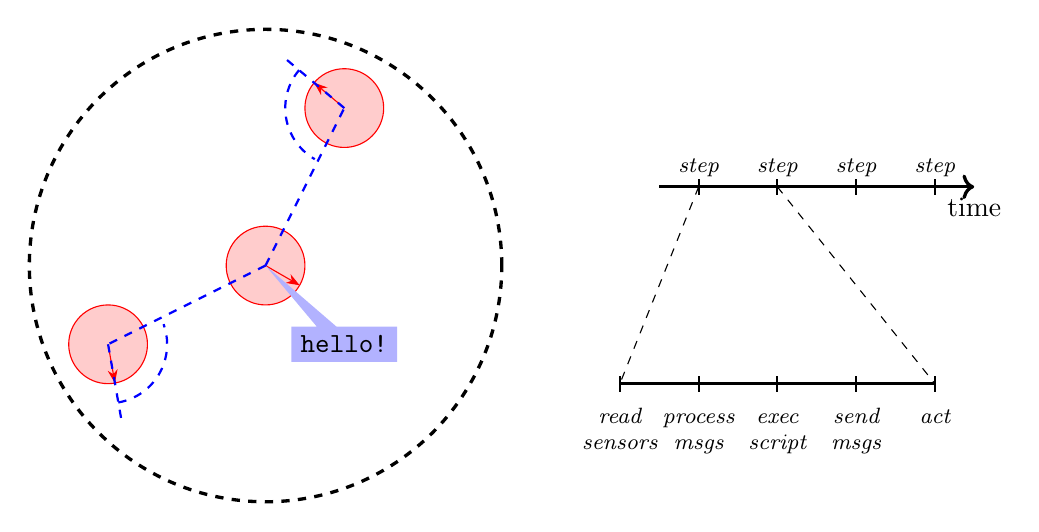
\begin{tikzpicture}
  % draw robots
  \coordinate(sender) at (3cm,3cm);
  \coordinate(recv1)  at (4cm,5cm);
  \coordinate(recv2)  at (1cm,2cm);
  \coordinate(point1) at ($(recv1) + (140:1cm)$);
  \coordinate(point2) at ($(recv2) + (280:1cm)$);
  \robot{sender}{-30}
  \draw[very thick,dashed] (sender) circle (3cm);
  \robot{recv1}{140}
  \robot{recv2}{280}
  \node[rectangle callout, fill=blue!30, callout absolute pointer={(3cm,3cm)}] at (4cm,2cm) {\texttt{hello!}};
  \draw[thick,dashed,draw=blue] (sender) -- (recv1);
  \draw[thick,dashed,draw=blue] (recv1) -- (point1);
  \draw[thick,dashed,draw=blue] ($(recv1)!.75!(point1)$) arc [start angle=140, delta angle=100, radius=.75cm];
  \draw[thick,dashed,draw=blue] (sender) -- (recv2);
  \draw[thick,dashed,draw=blue] (recv2) -- (point2);
  \draw[thick,dashed,draw=blue] ($(recv2)!.75!(point2)$) arc [start angle=280, delta angle=100, radius=.75cm];
  % draw stepping time line
  \draw[very thick,->] (8cm,4cm) -- ++(4cm,0cm) node[below] {time};
  \foreach \x in {8.5cm,9.5cm,10.5cm,11.5cm} {
    \draw[thick] (\x,3.9cm) -- ++(0cm,2mm);
  }
  \foreach \x in {8.5cm,9.5cm,10.5cm,11.5cm} {
    \node[above,font=\itshape\footnotesize] at (\x,4cm) {step};
  }
  % draw individual step time line
  \draw[very thick] (7.5cm,1.5cm) -- ++(4cm,0cm);
  \foreach \x in {7.5cm,8.5cm,9.5cm,10.5cm,11.5cm} {
    \draw[thick] (\x,1.4cm) -- ++(0cm,2mm);
  }
  \draw[dashed] (8.5cm,4cm) -- (7.5cm,1.5cm) (9.5cm,4cm) -- (11.5cm,1.5cm);
  \foreach \x / \t in {7.5cm/{read sensors},8.5cm/{process msgs},9.5cm/{exec script},10.5cm/{send msgs},11.5cm/{act}} {
    \node[inner sep = 0,minimum height=1cm,text width=1cm,text height=.25em,text depth=.25em, text centered,below,font=\itshape\footnotesize] at (\x,1.5cm) {\t};
  }
\end{tikzpicture}
\end{document}
